% TU Delft Beamer template
% Author: Maarten Abbink
% Delft University of Technology
% March 2014
% Version 2.0
% Based on original version 1.0 of Carl Schneider
\documentclass{beamer}
\usepackage[english]{babel}
\usepackage{calc}
\usepackage[absolute,overlay]{textpos}
% Side by side packages
\usepackage{graphicx,subfig}
% Change margin
\usepackage{changepage}
\mode<presentation>{\usetheme{tud}}

\title{MultiChain}
\subtitle{A cybercurrency for cooperation}
\institute[TU Delft]{Delft University of Technology}
\author{Steffan Norberhuis}
\date{December 14, 2015}

\setbeameroption{show notes}

\AtBeginSection[] % Do nothing for \section*
{
\begin{frame}<beamer>
\frametitle{Outline}
\tableofcontents[currentsection]
\end{frame}
}


%% Insert frame before each subsection (requires 2 latex runs)
%\AtBeginSubsection[] {
%	\begin{frame}<beamer>\frametitle{\titleSubsec}
%		\tableofcontents[currentsection,currentsubsection]  % Generation of the Table of Contents
%	\end{frame}
%}
%% Define the title of each inserted pre-subsection frame
%\newcommand*\titleSubsec{Next Subsection}
%% Define the title of the "Table of Contents" frame
\newcommand*\titleTOC{Outline}

% define a symbol which can be removed if you don't need it
\newcommand{\field}[1]{\mathbb{#1}}
\newcommand{\Zset}{\field{Z}}

\begin{document}


\setbeamertemplate{navigation symbols}{}

{
% remove the next line if you don't want a background image
\usebackgroundtemplate{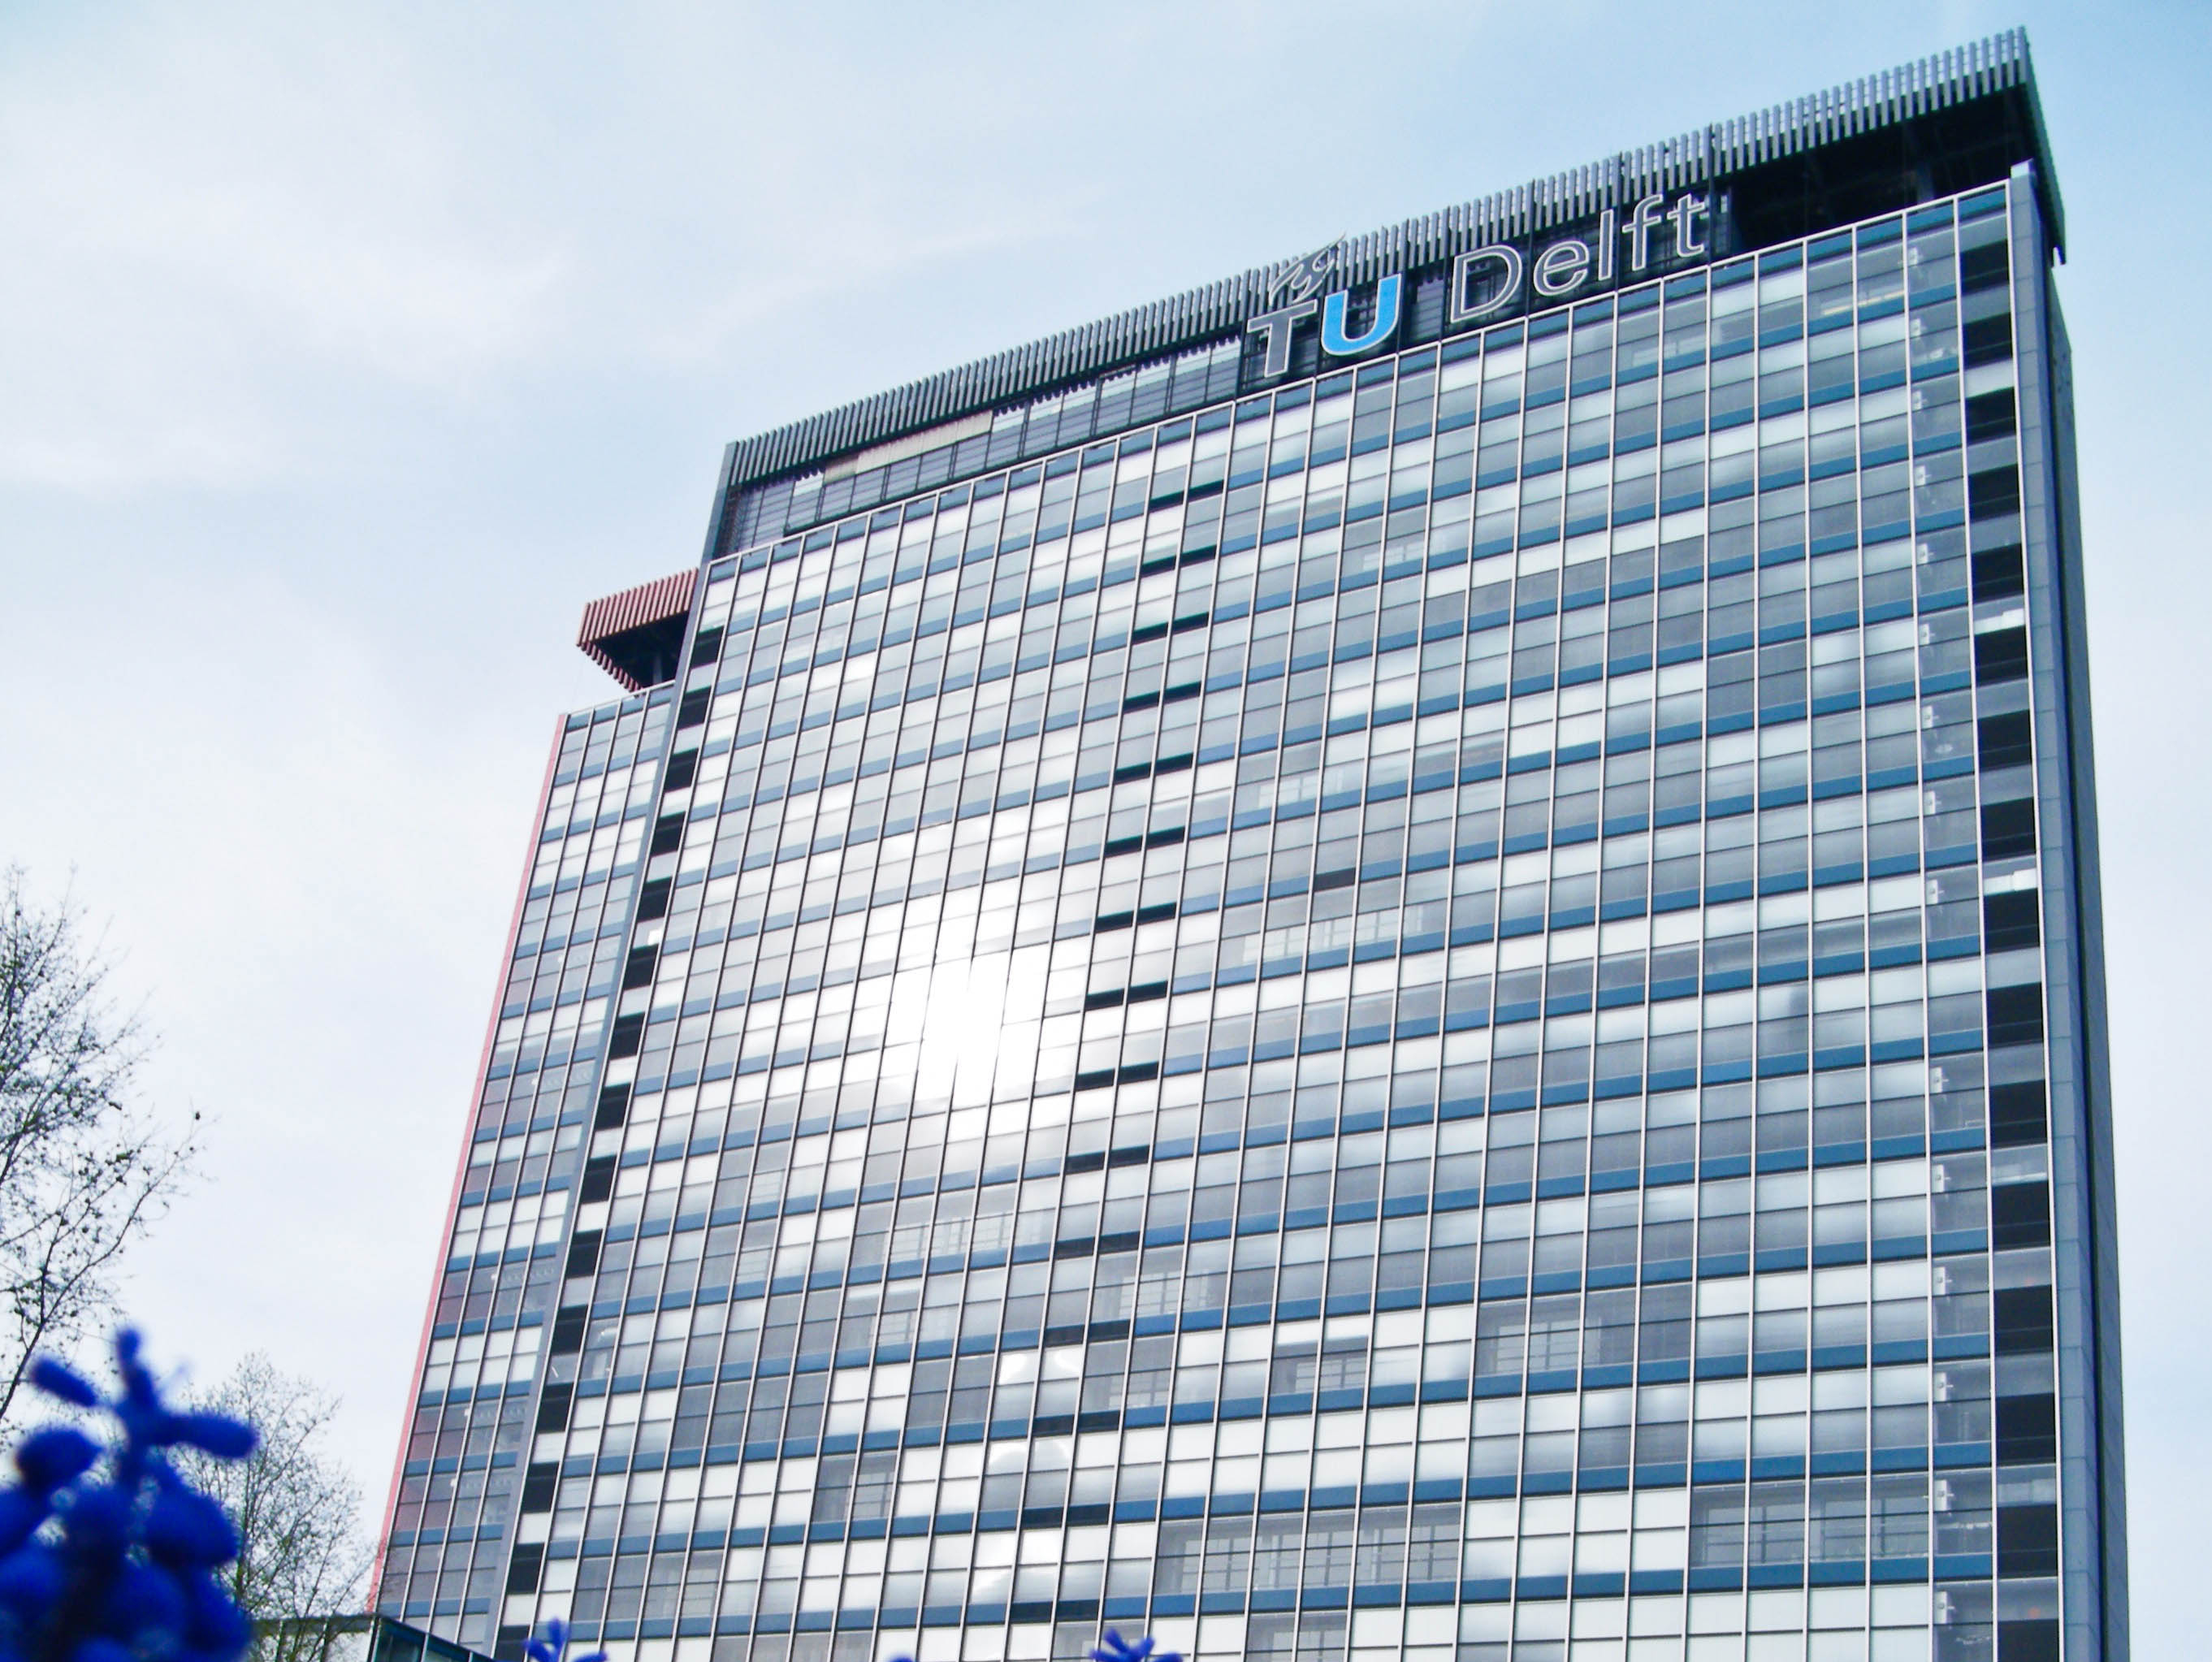
\includegraphics[width=\paperwidth,height=\paperheight]{images/background-titlepage.jpg}}%
\setbeamertemplate{footline}{\usebeamertemplate*{minimal footline}}
\frame{\titlepage}
}\note{
Welcome every one to my defence of my Master's Thesis.
The subject of my thesis is: MultiChain: A cybercurrency for cooperation.
For my thesis I contributed with a first step in a new cybercurrency.
This was done with the Tribler team at the TU Delft.
They develop a peer-to-peer filesharing program.
I will first tell you the outline of my presentation.
}

{\setbeamertemplate{footline}{\usebeamertemplate*{minimal footline}}
\begin{frame}\frametitle{\titleTOC}
	\tableofcontents
\end{frame}
}
\note{
I will start with describing you the problem that the new cybercurrency: MultiChain is trying to solve.
After that I will tell you about the design of MultiChain.
With MultiChain experiments were done to validate and test the system.
I will show you the result of these.
As this is a first step, some known vulnerabilities do exist and I will explain these.
Finally, I will conclude my thesis and describe future work.
}

\section{Problem Description}

\begin{frame}
\frametitle{Cooperation}
    \begin{definition}
		\emph{Cooperation}* is
		 \begin{itemize}[<+(1)->]
		    \item The action or process of working together to the same end.
		    \item Assitance, especially by complying readily with requests.
		 \end{itemize}
         \uncover<4->{
		    The essence of a collaborative, distributed system is that every node performs tasks for other nodes.
		    }
     \end{definition}
    \begin{figure}
        \centerline{
\includegraphics[scale=0.9]{images/problem/handshake.eps}}
    \end{figure}
    * source: The Oxford English Dictionary
\end{frame}
\note{
So lets start with the problem description.
As the subtitle mentioned, MultiChain is to improve cooperation in a peer-to-peer system.
Cooperation is defined as the action or process of working together to the same end.
It is giving assitance upon request.
And this is the essence of a collaborative, distributed system: every participant helps each other.
This system is open to join by any participant.
A peer-to-peer network is such a system.
}


\begin{frame}
\frametitle{Deciding to help}
    \begin{figure}
        \includegraphics<1>[scale=0.3]{images/problem/direct-reciprocity-1.eps}
        \includegraphics<2>[scale=0.3]{images/problem/direct-reciprocity-2.eps}
        \includegraphics<3>[scale=0.3]{images/problem/direct-reciprocity-3.eps}
        \includegraphics<4->[scale=0.3]{images/problem/direct-reciprocity-4.eps}
        \caption{\emph{Direct Reciprocity} between participants.}
    \end{figure}
    \uncover<5->{
        \begin{definition}
            The \emph{Free rider problem} is
            \begin{itemize}
                \item those who benefit from public goods, do not pay for them.
            \end{itemize}
            A private history prevents freeriding in a simple situation.
        \end{definition}
    }
\end{frame}
\note{
But participants do not always help.
Lets take two participants A and B as an example.
Participant A can decide to provide help to B.
And B can return this help.
But he can also choose to not provide this help.

B now benefits from the help of A without contributing.
The help of A can be seen as a public good.
I now have explained the problem of Free riding to you.
If A remembers that B does not contribute,
he can prevent the freeriding of B by not giving him help in the future.
So a private history can prevent freeriding in the future.

But most often interactions between participants in a peer-to-peer network are single, and help cannot be exchanged.
}

\begin{frame}
\frametitle{Help peers that help others}
    \begin{figure}
        \includegraphics<1>[scale=0.3]{images/problem/indirect-reciprocity-1.eps}
        \includegraphics<2>[scale=0.3]{images/problem/indirect-reciprocity-2.eps}
        \includegraphics<3->[scale=0.3]{images/problem/indirect-reciprocity-3.eps}
	    \caption{\emph{Indirect Reciprocity} between nodes.}
	\end{figure}

	\uncover<4->{
         \begin{definition}
             The \emph{Shadow the Future} prevents A, B, C from deciding not to help.
         \end{definition}
     }
\end{frame}
\note{
Again A can decide to help B,
but he will not want to do so if B never contributes himself.
A will only help peers that help others.
So he will only do that if B himself helps others.

In turn A will only receive help from C if he provided B with help.
This is based upon his reputation for helping B.
A,B,C will be fearful deciding to not help, if they will not receive help themselves in the future.
This is the Shadow of the Future.

But a peer-to-peer system is much larger!
}



\begin{frame}
\frametitle{Public history}
\begin{figure}
	\centerline{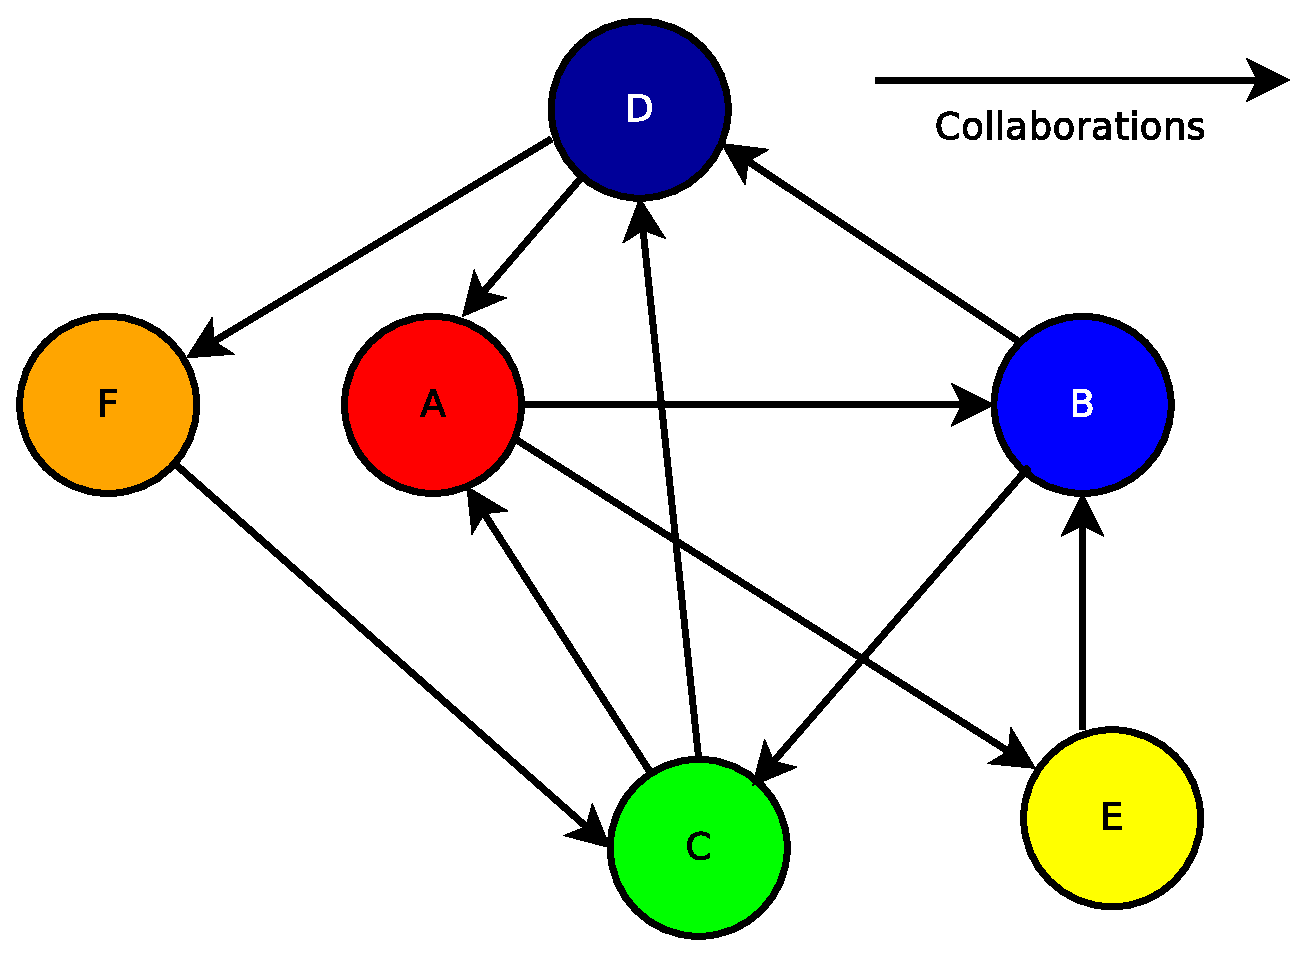
\includegraphics[scale=0.3]{images/problem/network-reciprocity.eps}}
	\caption{\emph{Network Reciprocity} between nodes.}
	\end{figure}
\pause
We need a public, tamper proof interaction history to incentivize collaboration and facilitate trust!
\end{frame}
\note{
You can have a whole network of participants connecting and providing help.
To still prevent freeriding the interactions have to be made public.
In such a network a participant can be malicious and we need to prevent his malicious behaviour.
We need a public, tamper proof interaction history to incentivize collaboration and facilitate trust!
So I now have described you the problem that MultiChain tries to solve.
}

\section{Design}
\begin{frame}
\frametitle{MultiChain}
  \begin{figure}
        \includegraphics<1>[scale=0.3]{images/design/multichain-1.eps}
        \includegraphics<2>[scale=0.3]{images/design/multichain-2.eps}
        \includegraphics<3>[scale=0.3]{images/design/multichain-3.eps}
        \includegraphics<4->[scale=0.3]{images/design/multichain-4.eps}
        \caption{MultiChain blocks chained together and becoming entangled.}
	\end{figure}
	\begin{itemize}
	    \item<2-> The blocks are chained using pointers hash.
	    \item<3-> The chain of A and C are entangled.
    \end{itemize}
\end{frame}
\note{
I will now explain to you the design of MultiChain.
The basis of MultiChain are blocks.
A and B will create a block together.
This contains the data about the interaction between A and B.
I will later describe the contents of the blocks.

This block can be retrieved and inspected by anyone by contacting A or B.
Using this information he will be able to decide to help A.

If A and B were to interact again they will create a new block.
This block is chained to the previous block using a hash pointer.
A hash pointer can be described shortly as cryptographic value that describes the block it points to.
Both A and B have an individual pointer that points to the previous block.
This is because A and B both have a chain themselves,
and the previous block could be different blocks.

A now receives help from C,
and A and C now create a block together.
This block will be chained to the previous block of A.
Now the chain of A and C is entangled at the new block.

Also B could interact with another peer D.
}

\begin{frame}
\frametitle{Block creation protocol}
\begin{figure}
	\includegraphics<1>[scale=0.3]{images/design/protocol-1.eps}
	\includegraphics<2>[scale=0.3]{images/design/protocol-2.eps}
	\includegraphics<3>[scale=0.3]{images/design/protocol-3.eps}
	\includegraphics<4>[scale=0.3]{images/design/protocol-4.eps}
	\includegraphics<5>[scale=0.3]{images/design/protocol-5.eps}
	\caption{Sequence diagram for block creation.}
	\end{figure}
\end{frame}
\note{
If A is the uploader he will initiate the block creation protocol with B.
He wants his contribution to be commit to MultiChain.
So he creates a message and adds his data and signature on this message.

He will send this message containing requesting to B add his signature to the block.

B will append his data and his signature. THe block is now created.

B responds with a message containing the block and will immediately add this new block to his chain.

When the message arrives at A he will also add it to his chain.

The block is now present in both chains.
}


\begin{frame}
\frametitle{Contents of a block}
\begin{figure}
    \begin{adjustwidth}{-1em}{0em}
    \includegraphics<1>[scale=0.25]{images/design/signatures-1.eps}
    \includegraphics<2>[scale=0.25]{images/design/signatures-2.eps}
    \includegraphics<3>[scale=0.25]{images/design/signatures-3.eps}
    \includegraphics<4>[scale=0.25]{images/design/signatures-4.eps}
    \includegraphics<5>[scale=0.25]{images/design/signatures-5.eps}
    \includegraphics<6>[scale=0.25]{images/design/signatures-6.eps}
    \includegraphics<7>[scale=0.25]{images/design/signatures-7.eps}
    \includegraphics<8->[scale=0.25]{images/design/signatures-8.eps}
    \end{adjustwidth}
	\caption{All 14 fields in a MultiChain block.}
	\end{figure}
	\uncover<9->{
	    \begin{definition}
	        Signatures have the property of non-repud.
	    \end{definition}
	}
\end{frame}
\note{
I will now describe to you the contents of a block.
First part is the up field.
This field contains the amount of data uploaded in MegaBytes by the uploader A.

The second part is the down field.
This contains the amount of data transferred back to A.

The public keys of A and B indentify A and B and are added to the block.

The total up and total down of A for the whole chain is added.

The hash pointer of A is added and a sequence number that identifies the block number in the chain of A.

This is all the added supplied by A.

Next, the total up and total down of B is added by B.

Also the hash pointer and sequence number of B is added.

The block contains the signature of A and B.
The signature of A is only on part of the block.
While B signs the whole block.

}



\begin{frame}
\frametitle{Half signed blocks}
\begin{figure}
	\centerline{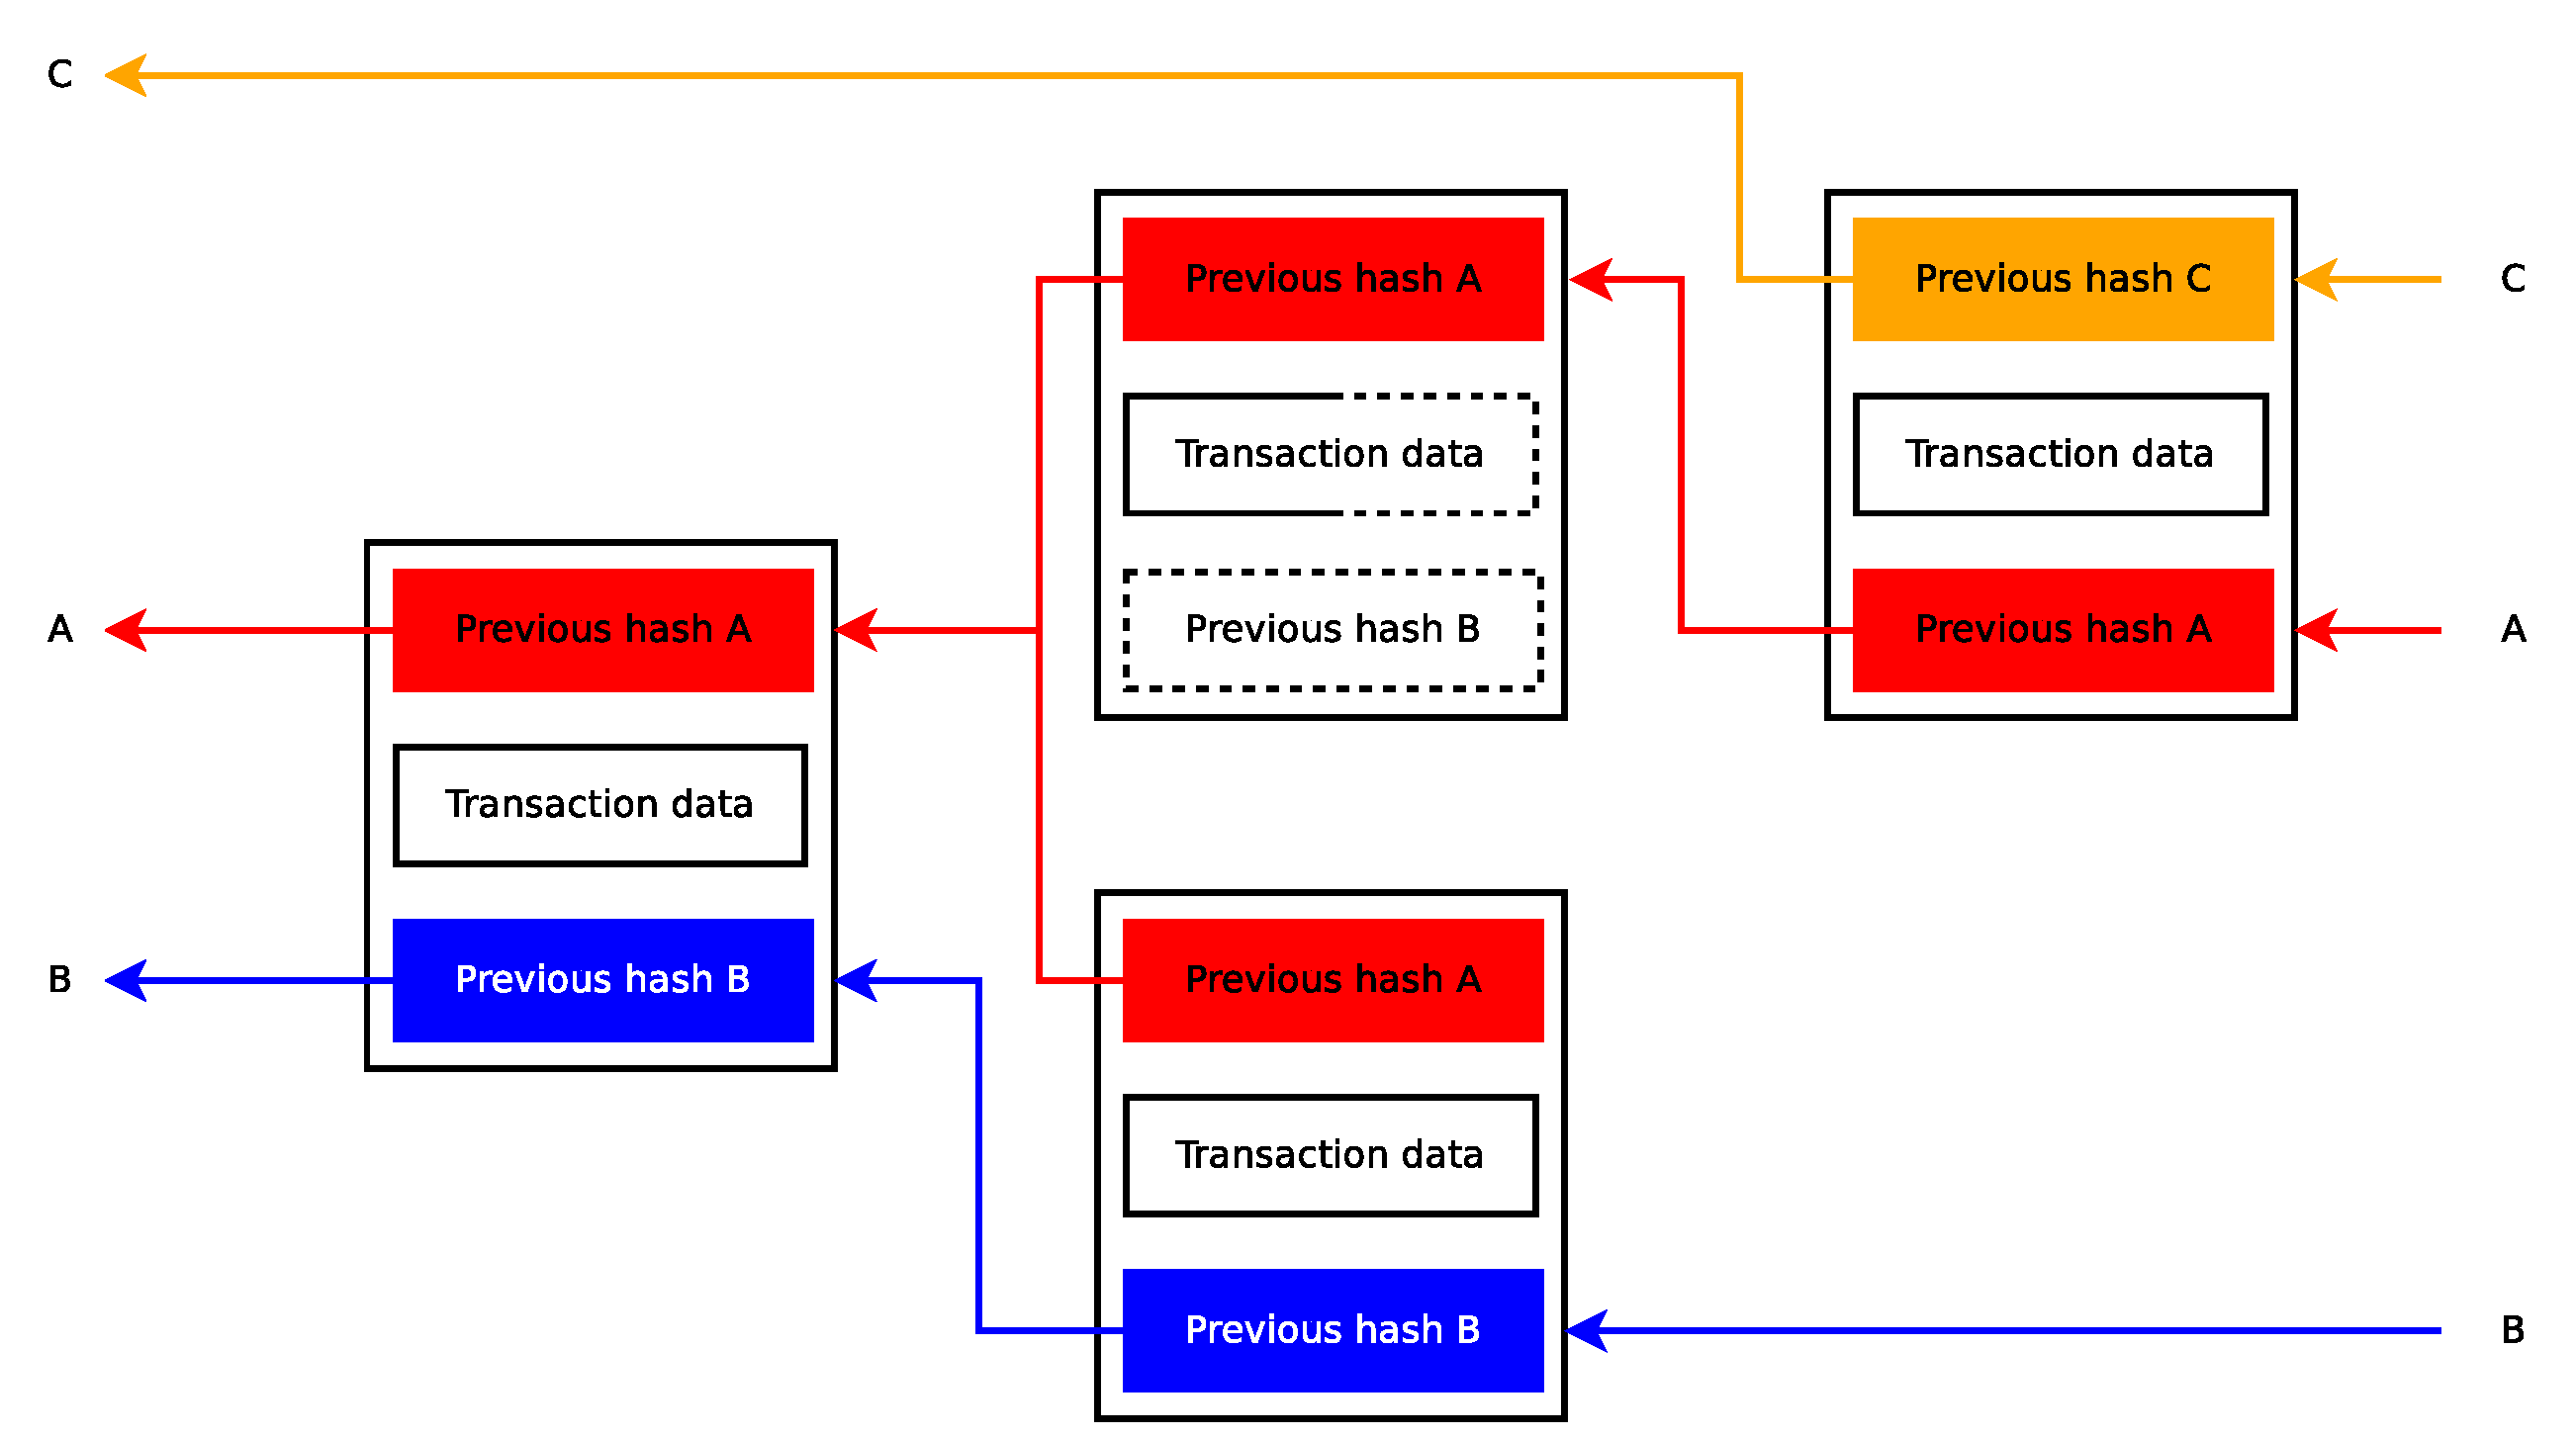
\includegraphics[scale=0.25]{images/design/halfsigned-chain.eps}}
	\caption{A chain of with a half signed block in MultiChain.}
	\end{figure}

\end{frame}

\section{Experiments}

\begin{frame}
\frametitle{Experimenting with chain creation}

\begin{figure}
\centerline{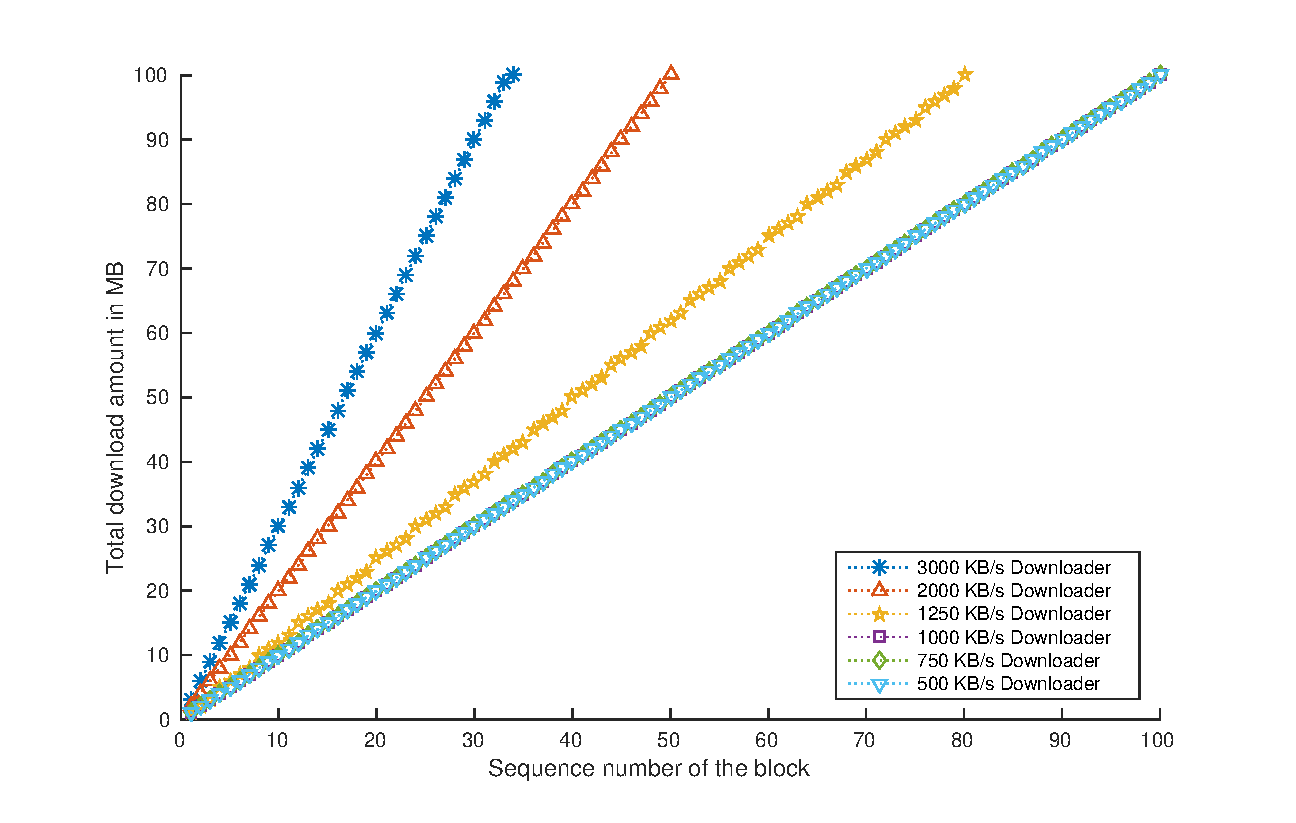
\includegraphics[scale=0.5]{images/experimentation/synthetic-simple-down.eps}}
\caption{Total download amounts repeated 6 times with different speeds.}
\end{figure}
\end{frame}

\begin{frame}
\frametitle{Anonymous downloading}

\begin{figure}
	\centerline{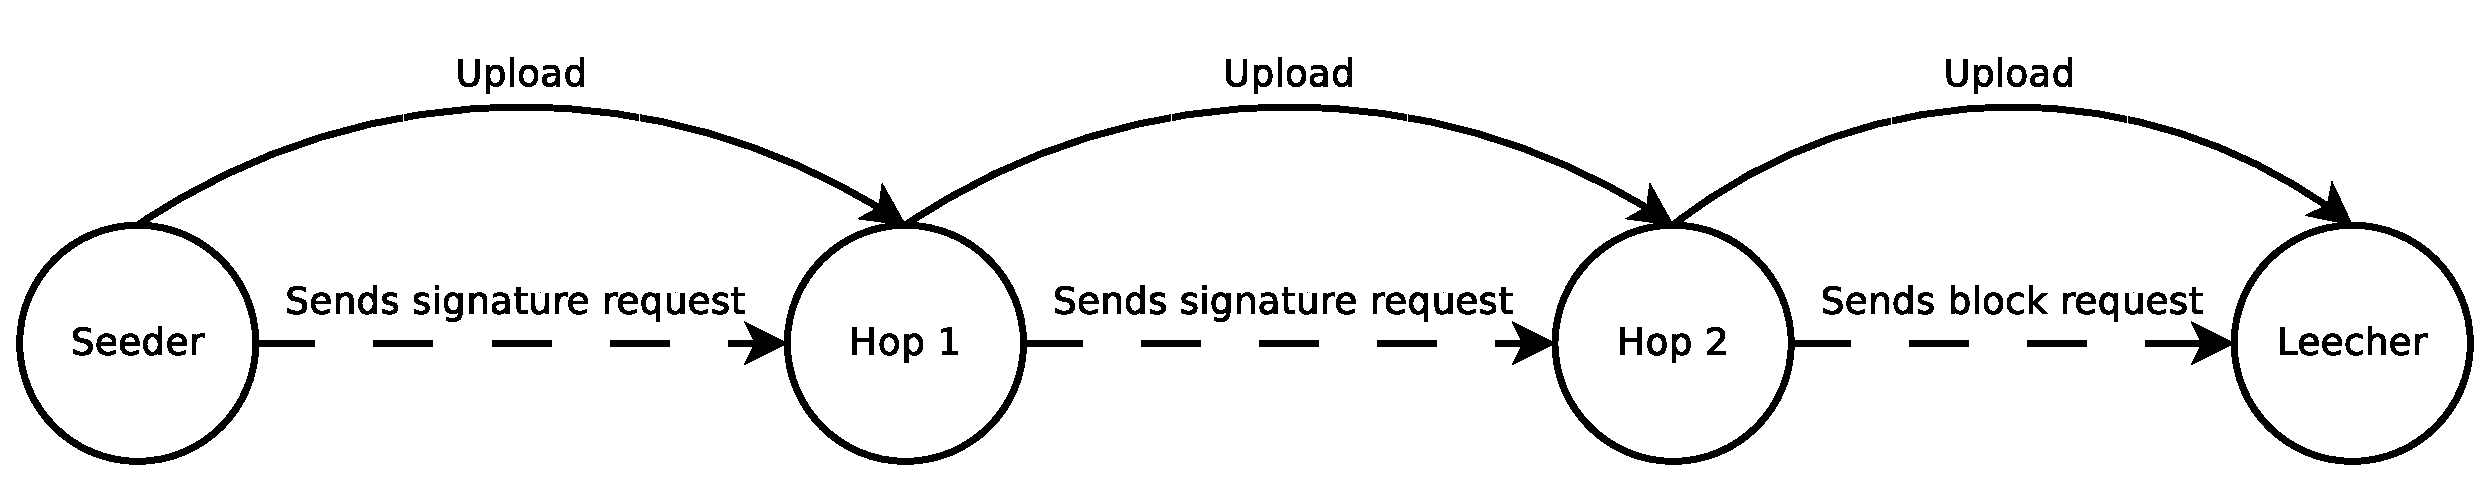
\includegraphics[scale=0.25]{images/experimentation/seeder-hops-downloader.eps}}
	\caption{Block creation in an anonymous download.}
	\end{figure}
\end{frame}

\begin{frame}
\frametitle{Anonymous download experiment}

\begin{figure}
    \centering
    \begin{adjustwidth}{-3em}{-3em}
    \subfloat[]{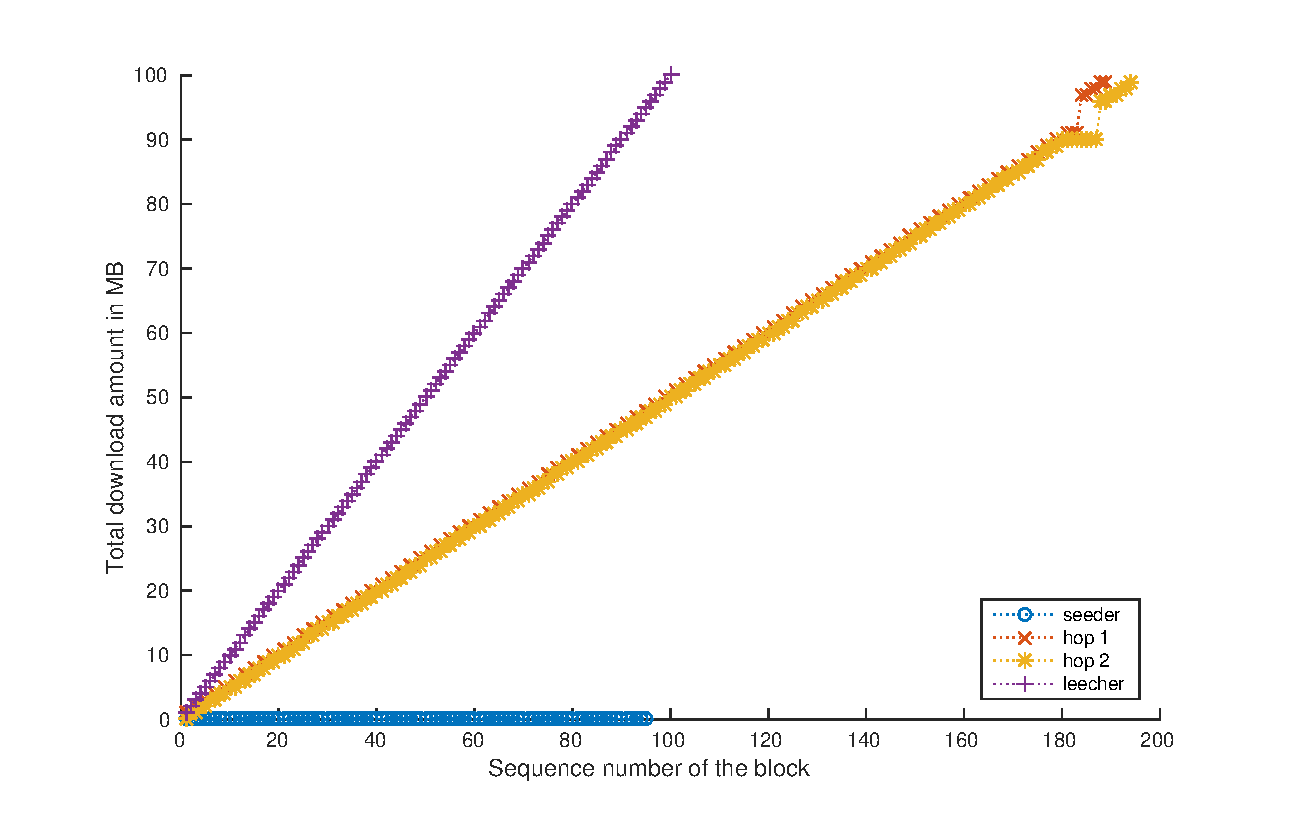
\includegraphics[trim={.5cm 0cm 0cm 0cm},clip=true,width=.46\linewidth]{images/experimentation/synthetic-anonymous-down.eps}}\hspace{0em}%
    \subfloat[]{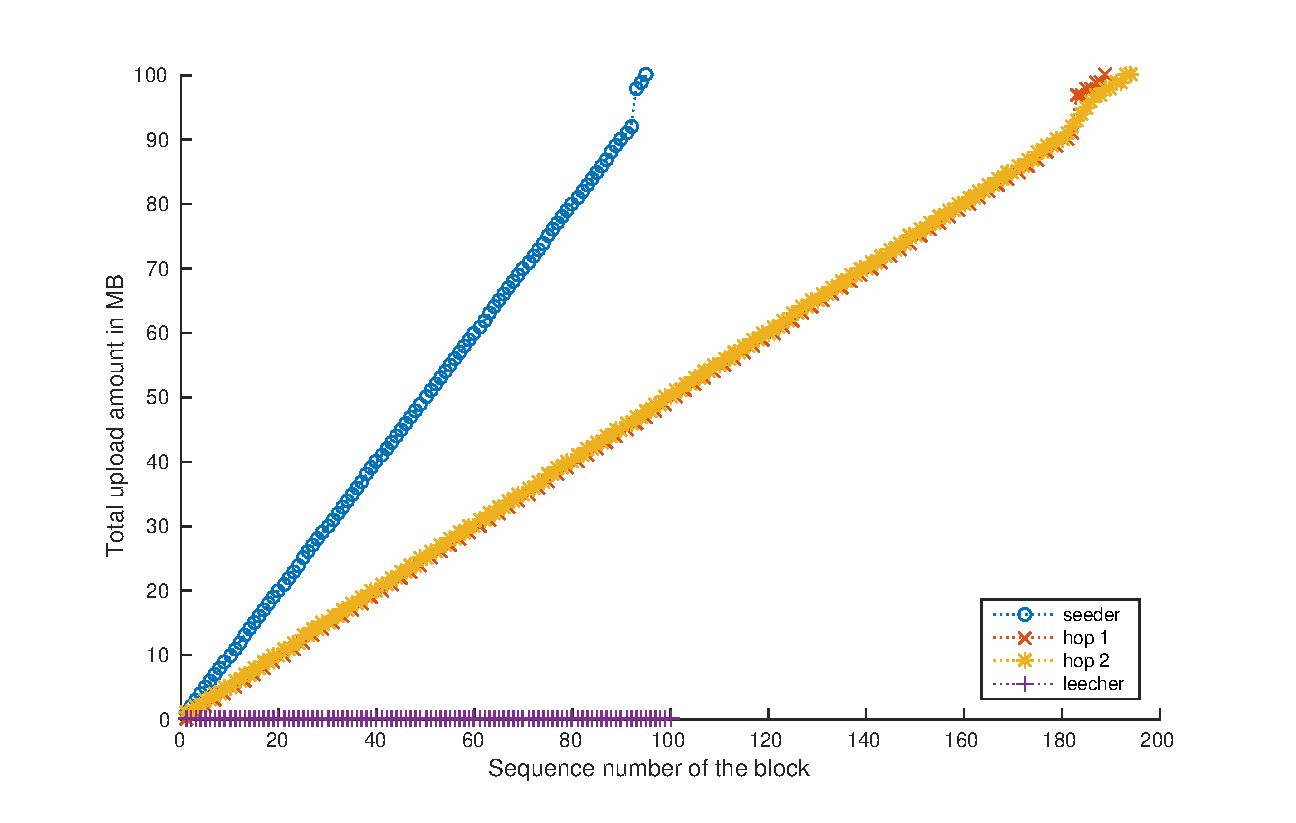
\includegraphics[trim={.5cm 0cm 1cm 0cm},clip=true,width=.46\linewidth]{images/experimentation/synthetic-anonymous-up.eps}}
    \end{adjustwidth}
    \caption{Download and upload amounts during the anonymous download experiment.}
\end{figure}

\end{frame}

\begin{frame}
\frametitle{Zooms of the MultiChain Graph}
\begin{figure}
    \centering
    \begin{adjustwidth}{-3em}{-3em}
    \subfloat[Entanglement]{\fbox{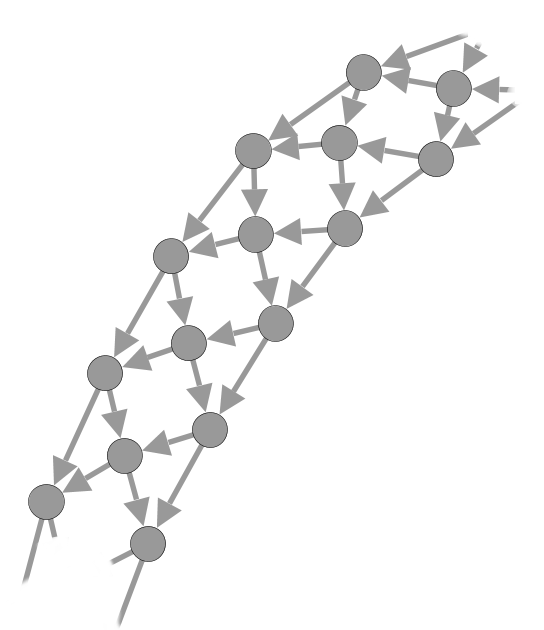
\includegraphics[trim={.5cm 0cm 0cm 0cm},clip=true,width=.46\linewidth]{images/experimentation/anonymous-magnified.png}}}\hspace{0em}%
    \pause\subfloat[Drop event]{\fbox{\includegraphics[trim={.5cm 0cm 1cm 0cm},clip=true,width=.46\linewidth]{images/experimentation/anonymous-timeout.png}}}
    \end{adjustwidth}
    \caption{Zooms of the entanglement and the drop event.}
\end{figure}
\end{frame}

\section{Known vulnerabilities}

\begin{frame}
\frametitle{Double spending}
\begin{figure}
	\centerline{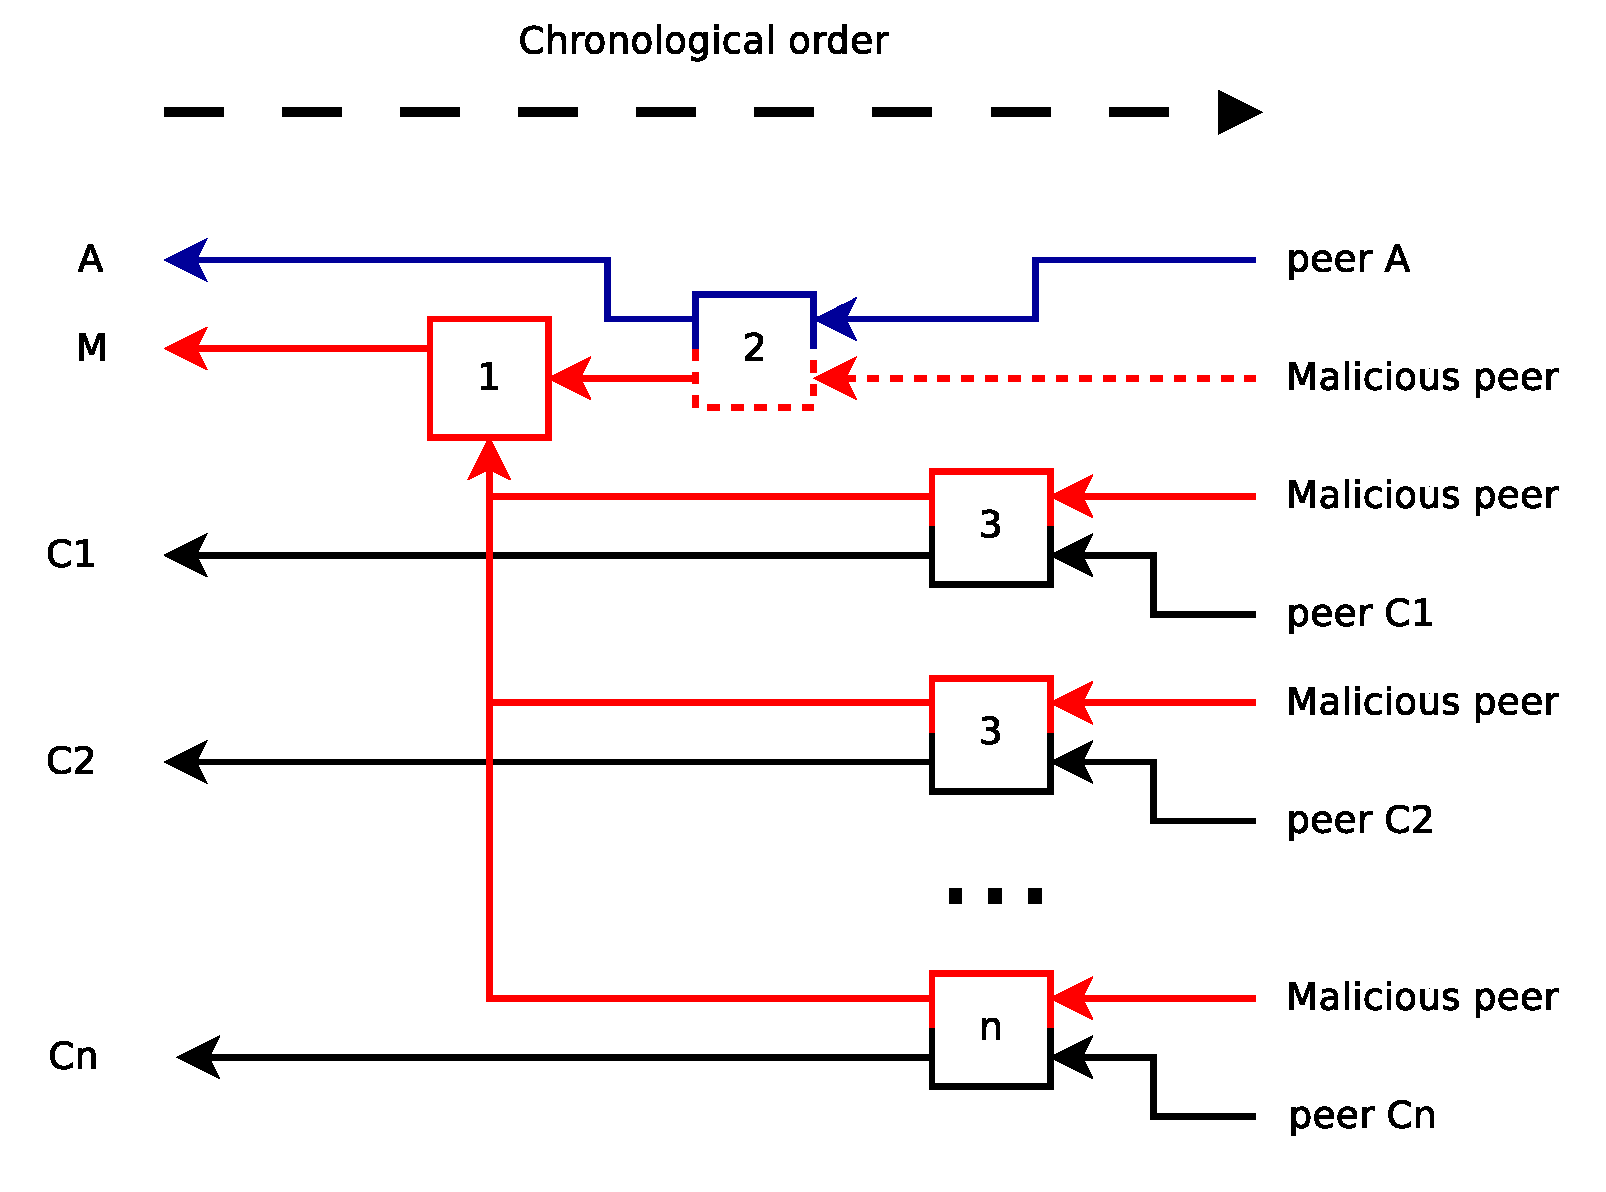
\includegraphics[scale=0.3]{images/vulnerabilities/branch-multiple.eps}}
	\caption{Double spending by M.}
\end{figure}
\end{frame}

\begin{frame}
\frametitle{Sybil attack}
\begin{figure}
	\centerline{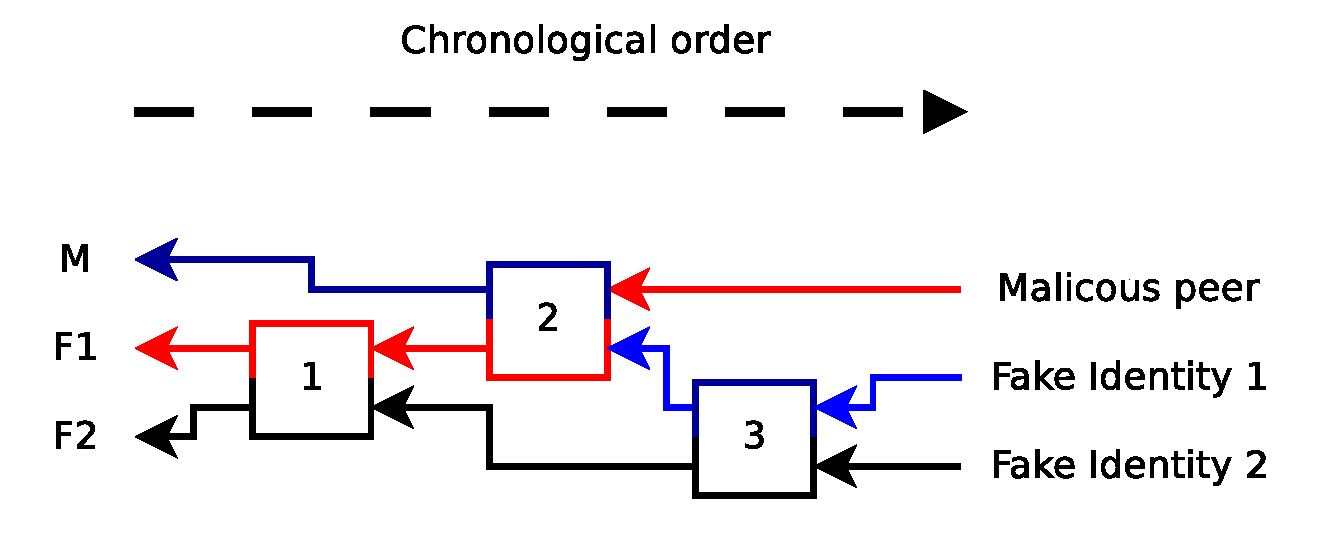
\includegraphics[scale=0.3]{images/vulnerabilities/sybil.eps}}
	\caption{The sybil attack by M.}
	\end{figure}
\end{frame}

\section{Conclusion}

\begin{frame}
\frametitle{Conclusion}
\begin{itemize}
\pause \item{Difficult to make a scalable reputation system. But a different approach can work.}
\pause \item{Experiments shows that MultiChain has promise to be a good replacement.}
\pause \item{A lot of work is still needed to provide adequate security.}
\end{itemize}
\end{frame}


\end{document}
